\chapter{Analyse des données}








\section{Data Mining - Exploration de données}

\subsection{Pre-processing}
%Description du dataset (rapidement, le reste dans un codebook)\\

%Mise en forme du dataset, une sortie à la fois vs plusieurs sorties etc \\
%On considère les données gustatives et les défauts physiques comme des sorties -> les prendre un par un ou tous ensemble\\

%Description du set, différentes parties des données, éventuelles données manquantes\\

Une grande partie de l'étape de préprocessing a été réalisée durant l'extraction des données. Il a en effet fallu extraire les données d'une manière uniforme et cohérente dès le départ afin de ne pas se retrouver avec des variables présentes uniquement dans certaines parties du set de données ou avec des variables incohérentes comme cela a été le cas de certains cafés qui avaient comme note de dégustation plus de cent points sur cent par exemple. Des éliminations ou des corrections ont été réalisées de manière automatisées ou manuelles afin de supprimer les erreurs. On notera parmi les corrections importantes le remplacement de virgules par des points, quelques erreurs de frappes (68.5 points sur 10 au lieu de 6.85 par exemple) ou encore des utilisations d'unités différentes. Le dataset résultant est décrit dans l'Annexe A de ce projet. Une fois cette étape de nettoyage réalisée, les premières informations ont pu être extraites des données.\\


\noindent Le schéma \ref{DatasetMaking} résume rapidement les différentes élimination d'observations au cours des étapes de construction du set de données. 

\begin{figure}[H]
	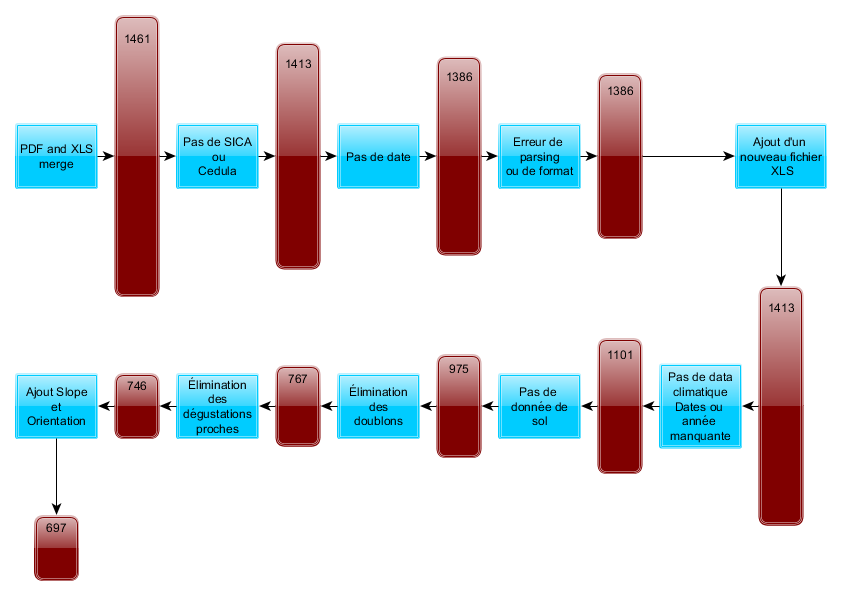
\includegraphics[scale=0.5]{Dataset_1}
	\caption{\label{DatasetMaking} Étape de construction du set de données et pertes d'observations.}
\end{figure}


\subsection{Corrélations entre variables}

Afin d'avoir une bonne vue d'ensemble sur les variables et leurs liens, les matrices de corrélation ont été calculées pour toutes les variables. Premièrement la corrélation entre les différentes sorties. Sur la figure \ref{correlation_sorties1} on peut observer que les défauts physiques des grains ne sont que très peu liés entre eux ou avec les résultats de dégustation. On remarque cependant que les données gustatives du café sont fortement liées entre elles. 

\begin{figure}[H]
	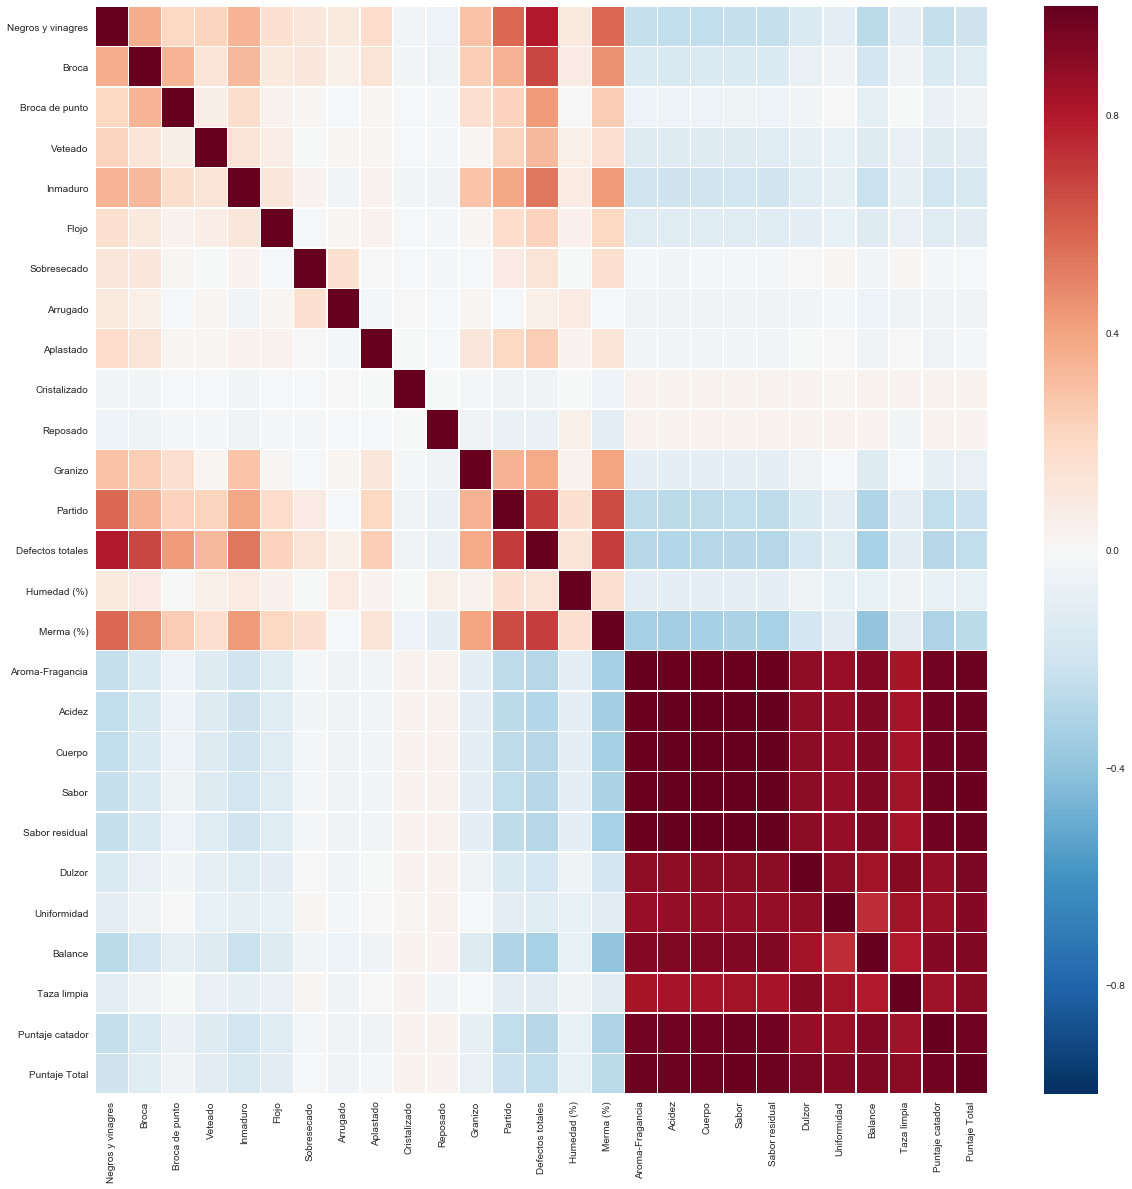
\includegraphics[scale=0.35]{correlation_sorties1}
	\caption{\label{correlation_sorties1} Matrice de corrélation entre les différentes sorties.}
\end{figure}


De la même manière, les corrélations sont calculées sur les entrées et sont visibles sur la figure \ref{correlation_entrees1.png}. 


\begin{figure}[H]
	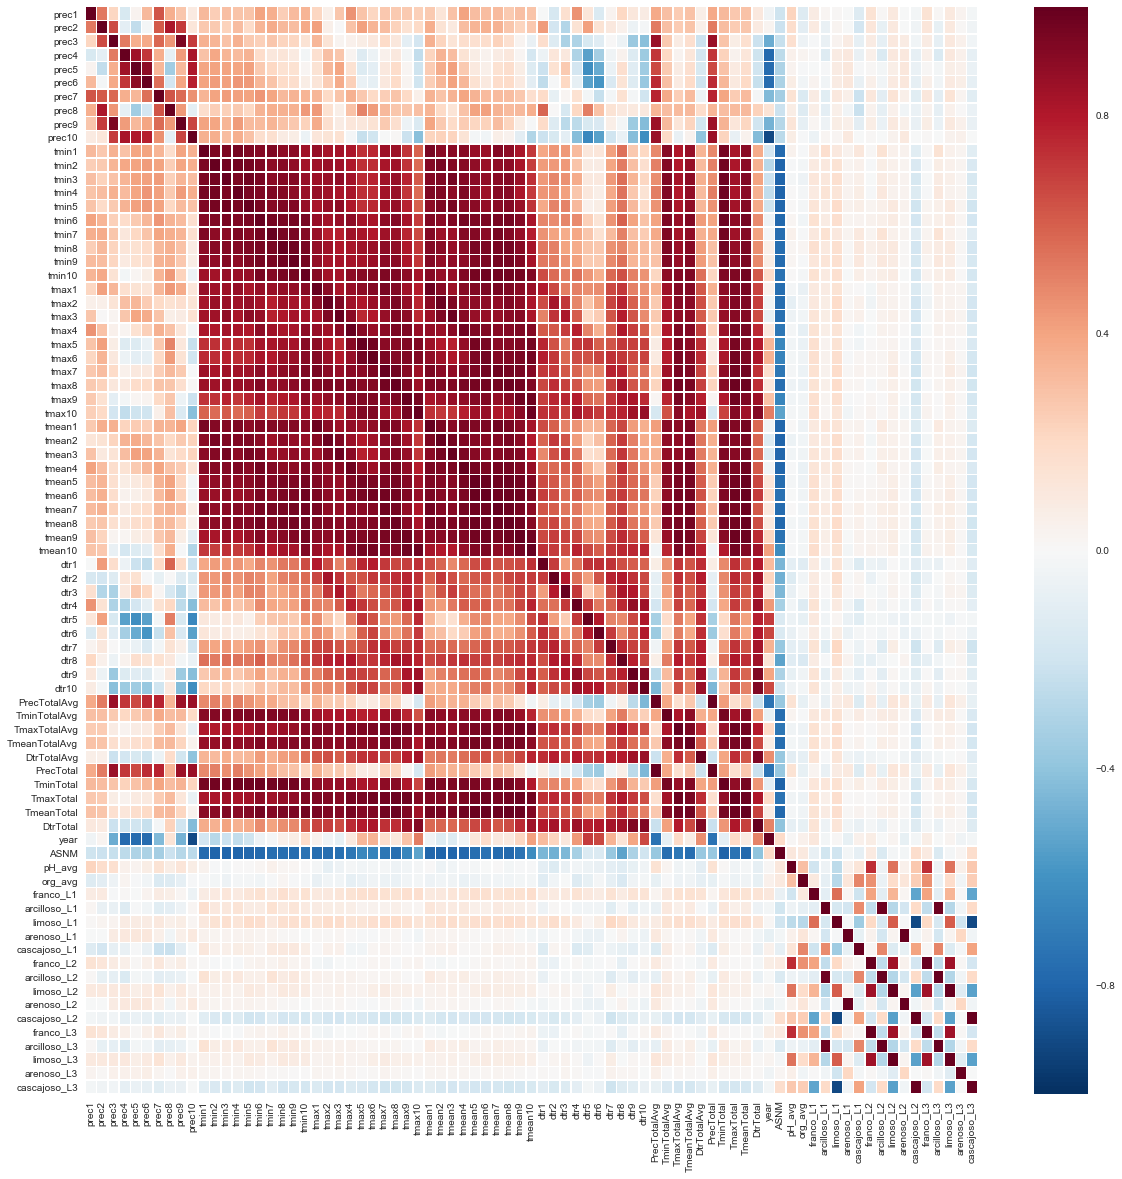
\includegraphics[scale=0.35]{correlation_entrees1}
	\caption{\label{correlation_entrees1} Matrice de corrélation entre les différentes entrées.}
\end{figure}


On observe que les données de sol sont parfois corrélées entre-elles mais presque pas du tout avec les données climatiques. On peut donc déjà soulever que le climat n'a pas ou peu d'influence sur la texture, le pH ou le taux de matière organique du sol des zones étudiées. L'altitude joue ici un rôle important par rapport aux données de température, ce qui reste compréhensible. 

%TODO garder un peu de place pour lorsqu'on ajoutera des données comme la pente, le soleil etc. 











\newpage
\subsection{Principal Component Analysis (PCA)}\label{PCAss}
La PCA, pour Analyse en Composantes Principales en français, est une méthode qui consiste à transformer un jeu de variables corrélées en nouvelles variables dé-corrélées les unes des autres. Ces nouvelles variables sont appelées composantes principales et permettent de rendre l'information moins redondante. Pour faire plus simple, l'utilité de la Composante Principale est de réduire le nombre de variables tout en gardant un maximum d'information. La figure \ref{PCAdefinition} montre une représentation graphique de la composante principale. 


\begin{figure}[H]
	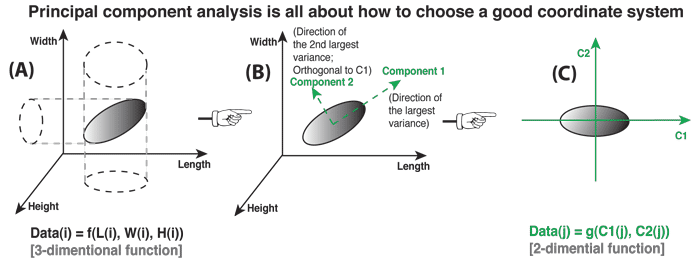
\includegraphics[scale=0.5]{PCA_1}
	\caption{\label{PCAdefinition} Description de l'Analyse en Composante Principale. (A) Description d'un objet simple de manière compliquée ( trois dimensions pour par exemple une ellipse en papier) (B) Trouver des nouvelles variables (axes de coordonnées) orthogonaux l'un à l'autre qui pointent dans les directions de la plus grande variance (C) Utiliser les nouvelles variables (axes) pour décrire l'objet d'une manière plus simple. }
\end{figure}

On pourra ici éliminer les variables n'ayant pas une eigenvalue suffisamment importante afin de se concentrer sur les variables les plus importantes afin de réduire le nombre de dimension du dataset. 



% https://georgemdallas.wordpress.com/2013/10/30/principal-component-analysis-4-dummies-eigenvectors-eigenvalues-and-dimension-reduction/


\paragraph{Observation de la PCA pour les variables climatiques et de dégustations} Les différents types de variables, c'est-à-dire les données climatiques (températures, précipitations) ou les données de dégustations, on été réduits un par un sur 3 dimensions afin de pouvoir les visualiser sur un graphique et d'observer les différences entre les deux années disponibles. Ceci permet de se faire une idée des différences.  

\begin{figure}[H]
	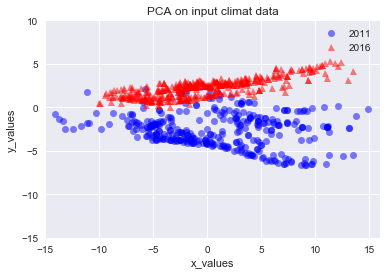
\includegraphics[scale=0.9]{PCA_Climat_All_1}
	\caption{\label{PCAClimatAll} PCA sur les données climatiques (Tmin, Tmax, Tmean, DTR et Prec) }
\end{figure}

\begin{figure}[H]
	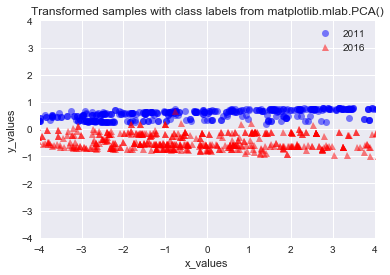
\includegraphics[scale=0.9]{PCA_TMEAN_1}
	\caption{\label{PCAClimatTmean} PCA sur les températures moyennes de chaque mois }
\end{figure}

\begin{figure}[H]
	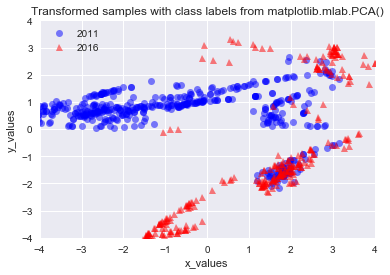
\includegraphics[scale=0.9]{PCA_PREC_1}
	\caption{\label{PCAClimatPrec} PCA sur les précipitations moyennes de chaque mois }
\end{figure}


\noindent Sur les figures \ref{PCAClimatAll}, \ref{PCAClimatTmean} et \ref{PCAClimatPrec}, on observe assez facilement deux groupes plus ou moins distincts se dessiner, un par année. On peut déjà en déduire que les deux années on été différentes sur le plan climatique. Afin de visualiser cette différence, nous pouvons observer la variation de la température maximale à Pereira, ce que nous montre la figure \ref{Tmax_Pereira} ainsi que la variation des quantités de précipitations, ce que nous montre la figure \ref{PREC_Pereira}. On observe une évolution commune entre températures (augmentation) et précipitations (diminution) qui nous rappelle l'influence d'El Niño sur le climat (Voir figure \ref{Nino}).

\begin{figure}[H]
	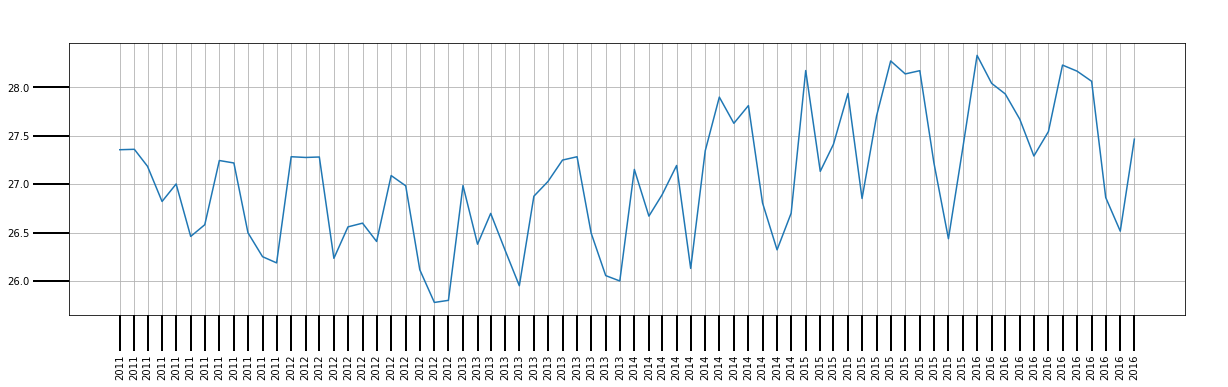
\includegraphics[scale=0.3]{Pereira_TMAX_2011_2016}
	\caption{\label{Tmax_Pereira} Variation des températures maximales à Pereira entre 2011 et 2016}
\end{figure}


\begin{figure}[H]
	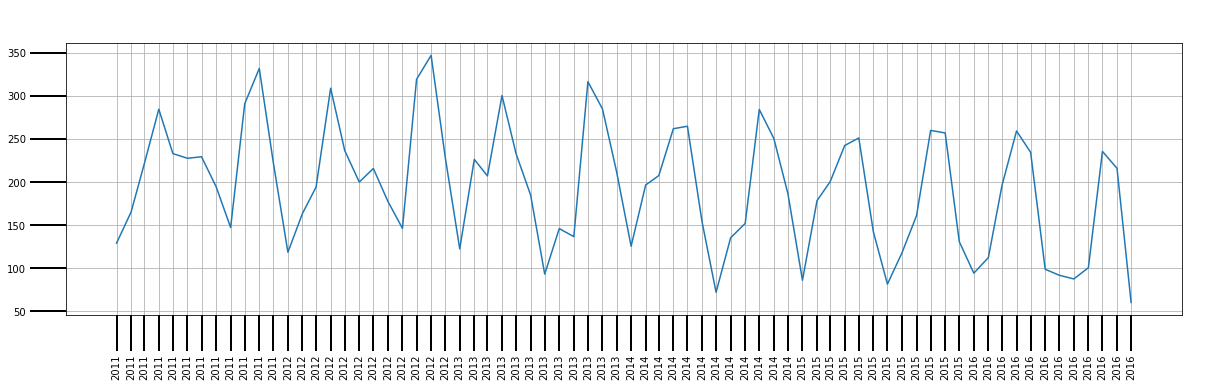
\includegraphics[scale=0.3]{Pereira_PREC_2011_2016}
	\caption{\label{PREC_Pereira} Variation de la quantité de précipitations à Pereira entre 2011 et 2016}
\end{figure}

\subsection{Self-Organizing Map}
%TODO 








\section{Prédiction}
%Il a été possible ou non de faire de la prédiction, confusion matrix etc
%ce que les méthodes comme random forest ont donné
Le but de cette section est d'analyser la possibilité de prédiction de la qualité des cafés à l'aide des données climatiques et de qualité de sols à disposition. Lorsque l'on parle de la qualité des cafés, on inclue autant les défauts physiques que les résultats de dégustation. 

\subsection{Random Forest}
% analyser des variables séparément. Possibilité de prédir les défauts vs le "gout", les défauts spéarément - les gouts séparément etc 



\chapter{Analyse des résultats}


%Analyse globale des résultats, discussion sur les résultats 
%Données manquantes

%Exemple: on sait que la fermentation du grain dans sa pulpe impacte sur la chimie de la graine et peut rendre le café plus ou moins acide -> pas de données sur la fermentation (temps, méthode etc) idem pour le séchage, le stockage, la récolte etc
